\documentclass[11pt, oneside]{article}   	% use "amsart" instead of "article" for AMSLaTeX format
\usepackage{geometry}                		% See geometry.pdf to learn the layout options. There are lots.
\geometry{letterpaper}                   		% ... or a4paper or a5paper or ... 
%\geometry{landscape}                		% Activate for for rotated page geometry
%\usepackage[parfill]{parskip}    		% Activate to begin paragraphs with an empty line rather than an indent
\usepackage{graphicx}				% Use pdf, png, jpg, or eps§ with pdflatex; use eps in DVI mode
								% TeX will automatically convert eps --> pdf in pdflatex		
\usepackage{amssymb}
\usepackage{graphicx}
\usepackage[nomarkers,figuresonly]{endfloat}
\graphicspath{ {images/} }

\title{Adapting Blog Readers for Multitouch}
\author{Willy Husted and Jackson Souza}
\date{11/25/14}							% Activate to display a given date or no date

\begin{document}
\maketitle

\begin{abstract}
The biggest challenge for multitouch blog reader apps is that they ignore often desired features found in dedicated longform devices such as e-readers and, most importantly, paper books. This means that current apps fail to fully utilize touch gestures, opting to recycle point and click interaction found in their web-based counterparts rather than capitalizing on similar dynamic touch interaction found in books and e-readers.
\end{abstract}

\section{Introduction}
In a 2006 letter to Oprah, Harper Lee, of \textit{To Kill A Mockingbird} fame, wrote, ``Can you imagine curling up in bed to read a computer? Weeping for Anna Karenina and being terrified by Hannibal Lecter, entering the heart of darkness with Mistah Kurtz, having Holden Caulfield ring you up---some things should happen on soft pages, not cold metal.'' \cite{Lee} In an age of boundless information with technology emerging to support ``book-like'' reading, we see similar sentiments cropping up. Current avenues of reading for an increasingly younger population are shortform, which is historically read on cold metal. The most intuitive devices we have that ``compliment" reading are designed around the way writing is presented on the web: short, sweet, and to the point. Many objections to the interaction styles and design that surround shortform writing for book-sized devices are concerned with the fact that they radically depart from the intimacy of reading a book. Untangling these emotionally charged views is difficult, but at the heart of the issue lies unfamiliar interaction with shortform content. Blog reader type apps fail to fully utilize touch gestures, opting to recycle point and click interaction found in their web-based counterparts rather than capitalizing on similar dynamic touch interaction found in books and e-readers. 


\section{Related Issues and Context}

As discussed above there are three major areas from which scrutiny about modern reading devices come from. One debate is ``shortform writing vs. longform writing'', which is in part what Lee is talking about in the initial quote. This issue is what motivates the other two, and is not necessarily addressable by altering an interaction style. Books inherently carry a story which communicates value and sparks the imagination, and for the past thousand-odd years, this has been the primary source through which we interact with written content. Reading is no longer synonymous with the longform, nor the book, and the seeming departure of a cherished meaning from the most frequently consumed written work irks many people.

The evolution of reading devices from dedicated devices such as the paper book and e-Reader to multifunction devices (laptop computers, iPads, etc.) serves as the ``jumping-off'' point for the issue at hand. Multifunction devices that simulate touch currently have the potential to bear the most likeliness to books, and mainly support shortform content. This is representative of the dilemma of Lee and many others: interaction on reading-centric apps is focused on supporting the shortform. So, this begs the question: can we match or exceed the interaction style of the paper book or dedicated e-reader to create a more meaningful reading experience with longform content?

Multitouch devices have the ability to mimic books, but, unfortunately, much of the design borrowed for reading apps are from devices non-conducive to touch, such as older e-Readers and web-based RSS readers. Apps like Flipboard represent a growing trend to provide a user with unique content and a friendly interface, preserving some of the sacred ``meaning only found in books.'' Interaction design research says we can push this design further.

\section{Design Implementation}
Joan Vinall-Cox explains in her article ``Moving from Paper to E-Book Reading'' that, ``The reading that occurs when people scan Web pages or engage with social media requires massively different eye-pattern movements and intake-and-response habits than the reading of books. [On the other hand], the reading of books requires eyes moving only from left to right (for English), sustained attention, and the ability to follow the author's (hopefully well-written) train of thought: A different set of reading habits than on websites...'' \cite{vinall-cox} Despite her personal use of a multitouch e-reader, Vinall-Cox feels that the set of gestures provided by the app are disgenuous, either in performance or in congruency to ``reading response'' habits. She elaborates on her e-reader's highlighting function, where she is able to select text and copy it to a collection of quotes. In order to complete this action, she must complete many steps besides the initial gesture of highlighting. Selecting the highlighter from a toolbar, choosing what collection to file the quote in, and validating the selection are all steps that Vinall-Cox believes remove the reader from the immersion of the content.

This does not only happen with dedicated longform devices, but in fact is most pervasive in shortform reading on the web or in apps. Multitouch does much in the way of (potentially) eliminating a cluttered interface of buttons and entry fields, mirroring the simplicity of paper. Yet, blog reader apps still rely on these interaction methods for navigation and content discovery. Content sharing and saving are often represented on a toolbar as ``+'' and ``Save''. Discovery and article selection are always represented in a list. As Jesse Burstyn comments, ``While not necessarily the most efficient, techniques such as folding and flipping pages are ingrained gestures that are lost with this new medium'' \cite{Burstyn}.  Clearly, a reconciliation of features is needed.

In our design, we were able to distill the primary features of the top three blog reader apps and modify them according to current interaction design research with attention to promoting a more pleasurable reading experience. In the three apps---Newsify, Feedly and Flipboard---we found that there were four main areas of focus: Article and Post Navigation, Content Discovery, Content Saving or Clipping, and Sharing. 

In the following sections, we will present these areas and tell how they were addressed in the three apps, making sure to include challenges and barriers to entry. Then, we will show and elaborate on our research-backed implementation of the areas within our design. Justification of the mockups in the greater context of interaction design will be given in section 4.

\subsection{Navigation}

\subsubsection{Article Navigation}
We begin with an obvious difference between typical multifunction and dedicated reading interfaces: in the former, text is typically laid out in a vertical arrangement. The arrangement of the text necessitates a downward scrolling, where in dedicated longform apps and devices, pages are usually flipped horizontally. In all three apps, the vertical scroll is upheld, with the notable exception of Flipboard, who implements a wall-calendar like ``flipping'' of the article. Flicking up folds half of the screen to reveal the next ``page'' of the article. 

In Jesse Burstyn's analysis of navigation implementations in e-readers, he says the following: ``In many cases, these [navigational] motions [in books] were so automatic that partial or even complete page flipping occurred prematurely; gaining subtle peek of the contents on the next page. Contrast this with existing e-book readers where navigating between pages is an intentional act of pressing a dedicated directional button'' \cite{Burstyn}. In attempts to solve this issue, Burstyn altered the shape of his proposed device. Yoon et. al. was able to implement a similar navigational technique, opting for a flat screen with the ability to flip through pages quickly or ``peek'' at the next.

Through the research, it is apparent that the sought after difference between paper and ``cold metal'' concerning navigation of a single piece of writing is the ability to rifle or skim through pages quickly, peek ahead, and return to the previous pages. In our design, we chose to utilize a full flipping animation to promote ``peeking'' (See Figure \ref{fig:Flip-1}), where the user physically pulls the page back, horizontally. To promote quick ``rifling'' through a longer article, the user can pull right to left with three fingers, skipping three pages at a time, while still being able to peek at their contents. (See Figure \ref{fig:Flip-2})

\subsubsection{Post Navigation}
The other main type of navigation between the apps is where the user selects their article to read. Strikingly similar to web based RSS readers, these views were comprised of a list, with Newsify being the most cluttered. Feedly opts for a single column list, including (like the others) the title, a photo, and small excerpt of an article, which then needs to be selected by a user. Alternatives for navigating through a collection of text are not usually found within longform devices. The closest counterpart would be a table of contents or search function in an e-reader.

Regardless of the interface, writing is often divided into sections and those sections are made easily accessible by a representation as a list. Because there is not necessarily any issue with this design, we reiterated it in our dream layout. Combining the features from Feedly (not cluttered, endless list) and Flipboard (large list items) in our design allows the user to quickly find an article to read, with a full width list, large excerpts and minimal clutter. Endless vertical scrolling (See Figure \ref{fig:endless-scroll} ) allows the user to skip large parts of the list, a feature that was deemed desirable in the previous section.

\subsection{Content Discovery}
All of the apps presented interesting ways to discover new content, which was then featured on the ``post navigation'' list. Feedly and Flipboard present the user with a Twitter-like hashtag system. In this system, the user indicates (via text input) his or her interests, or, alternatively, selects categories that he or she might be interested in. In dedicated devices, similar linkage to other resources would only be found in an index or bibliography. Even then, the resources would be restricted to the subject matter contained in the work.

Mitigating text input and an ``index-like'' list were our primary concerns in our design. In Veras et al's ``Interaction for Reading Comprehension on Mobile Devices'', the researchers proposed a tool that would highlight words in an article corresponding to that user's vocabulary. They saw this feature as conducive to breaking down an intimidating wall of text. A similar feature developed by Tashman and Edwards allows the user to highlight and save words in hopes of increasing vocabulary.

In our design, we thought that the act of accessing new content  should be developed in a similar vein, where the user is able to indicate words that corresponds to his or her interests. This is done inside the article view with a pinch gesture on the specific word or phrase (See Figure \ref{fig:Saving-Pinches}). The user can also ``zoom'' or reverse pinch to negate words and indicate topics they do not want represented in their recommended reading.

\subsection{Saving}
The equivalent to ``dog-earring''  a page in multitouch blog readers is when a user adds a post or article to a personal ``collection''. The user is then able to access the article or text clipping at any time by navigating to his or her collection. A feature unique to Flipboard is that this collection optionally becomes public as a ``Magazine''. In the article view, this action is usually represented by a ``Bookmark button''.


Dog-earring specifically was brought up again and again as a hallmark feature of what makes a book's interactivity so satisfying to a user. Rosner et al make the following observation about bookmarking: ``Changing material properties of objects can take advantage of our tactile memory, or subtly draw attention to an object, helping people find information more easily. [A developer should] provide ways for users to temporarily alter the physical medium of an interface'' \cite{Rosner}. The corollary to the dog-ear in shortform is the bookmark. Our gesture-centric implementation of bookmarking reiterates the dog-ear, dragging with one finger from the top right to save a page and with two fingers to save an article. See Figure \ref{fig:dog-earring}

\subsection{Sharing}
Flipboard's ``Magazine'' represents a community-centric way to share reading lists with the added option of exporting an article or the list as a whole to social media. Feedly and Newsify opt for a ``Share with [social media, email]'' button. Content sharing is a function unique to multifunction devices. In our design, we sought to mimic Flipboard in merging the bookmark and share functions. Every dog-ear a user makes is saved to his or her collection, and, similar to Flipboard's Magazine, that saved content is then made public. Direct social media sharing of an article or quote removes from the immersion of the material, so we sought to design a hands-off way to share.

\section{Usage Scenarios}
\subsection{Native Newspaper App (Medium Length Writing)}
One use case for our system is a newspaper's native tablet app, such as the New York Times. Our gesture based system (swiping with one finger, swiping with multiple fingers, dog-earring from the corner) would thrive on the medium-sized screen of an iPad or any other multitouch tablet. The tablet size would be preferable to an average current phone size (5 inches or less) because the smaller a screen, the more difficult multitouch gestures like three-finger swiping would become.

Another argument in favor of using our design in a native tablet app is that we tailored the concept of Post Navigation to look best on a tablet platform. A New York Times native app could take advantage of the paper-sized screen of a tablet to allow for greater familiarity to a physical newspaper. The New York Times could also benefit from our choice of endless scrolling to go beyond the limitations of a physical newspaper by allowing the user to access past articles from days, weeks, or months ago.

\subsection{Twitter Client (Short Length Writing)}
Another use case for our system is a native Twitter client on iOS and Android phones, two systems that support the multitouch gestures we take advantage of in our design. Some features of our system are already utilized by most Twitter clients---including the original client designed by Twitter. One such feature is the endless scrolling we adapted for Post Navigation. 

Other features, though, could increase the satisfaction and efficiency metrics for an updated Twitter client. One instance is our method of Content Discovery. When browsing our updated Twitter client, users would be able to pinch with two fingers on specific words or phrases to indicate interest in a topic. Then, our Twitter client would be able to search on that word or phrase for tweets on the same subject. For example, a user watching a football game could pinch the word ``football'' and receive a list of related tweets. This is an upgrade from the current Twitter client because our Content Discovery would expand beyond hashtags. A user can search on a word that is not a hashtag, allowing for greater breadth of search. Furthermore, searching on phrases instead of single words or hashtags (an extended form of one word) would allow for a similar greater breadth of search. A better search function obviously relies on backend work done by Twitter, but, assuming the backend allowed it, our gesture based search would increase satisfaction and efficiency for a native iOS or Android mobile app.

\section{Design Justifications}
Our main concerns in developing our layout were: restoring simplicity in the all views (esp. reading views), combating any removal from content immersion, and restoring touch-centric interaction found in paper books.

Pages in a book have what is referred to in interaction design as a ``natural mapping''. This term is used to describe the constraints of particular interfaces that allow users to easily infer necessary information about the system. For books, the mapping lies in the simplicity of the pages, and boundless amount of ways to manipulate the paper itself. Initially, we were concerned that restoring simplicity in the interface would lead to a lack of affordances. Many recent, more ``cutting-edge'', multitouch apps are guilty of this, for example, employing hidden sidebars accessible only with swipe left and right gestures. Hiding is a fantastic way to institute simplicity, but hidden features require a tutorial, and thus a learning curve. Books are intuitive enough to be simple and easy to use as a result of their natural mapping. In the article navigation and saving features, we mimicked common features from books such as dog-earring and page flipping. Retaining the natural mapping of books mitigates many of the complaints concerning the usability of ``cold metal''.

We were able to enforce simplicity within the app by automating many of the repetitive tasks, such as sharing and content discovery. In Flipboard, Feedly, and especially Newsify, simplicity in these actions seemed to be directly correlated to the amount of error-proneness. For example, sharing with Feedly requires the user to select from several social networks in a small menu, login to the selected social media account, select what to share, and then actually post the message to his or her account. Conversely, in the initial setup of Flipboard, the user is able to select immediately which networks to share their Magazine with. After linking to a social media, sharing becomes much more efficient because there are less buttons to press, and, therefore, less time to complete the task. Similarly, the "link once" design is also less error prone because less buttons to press means less potentially incorrect buttons to press. We sought a similar implementation in our app, with our dog-earring feature. Using this gesture for bookmarking allowed our design to keep within the natural mapping of the paper book, eliminating any potential learning curve and thus increasing learnability.

Added simplicity takes place in our removal of many input fields, mainly in the area of content discovery. The slight addition of any input fields would automatically conflict with the natural mapping of the book, as it is a passive object. The pinch in and out feature lets the user ``actively read'' while not removing them from the immersion of the content. A positive effect of reinterpreting many features to better represent a multitouch interaction style is that gestures also enforce consistency. When features of an application are implemented as gestures, interaction becomes uniform across a user base. This consistency is crucial for increasing proficiency in new users. Similar to the conclusions in the paragraph above, it would be inconsistent with the natural mapping of the book to remove the reader from immersion by forcing them to remember actions unique to their settings. We chose to side heavily with automation, because successful dedicated reading devices perform few actions other than displaying text.

\section{Usability Metrics}
\subsection {Learnability}
Learnability will generally be a strong metric for our design because many of the interactions are based on physical books, a system everyone literate is familiar with. Prior knowledge of how to turn a page translates well to our system. More concretely, our design is highly learnable because it relies on direct manipulation. Direct manipulation is an interaction style that involves ``rapid, incremental, and reversible operations whose impact on the object of interest is immediately visible.'' \cite{Kwon} In our system, turning a page and dog-earring are two examples of interactions that utilize direct manipulation. This style choice improves learnability because of the ``Layered or spiral approach to learning that permits usage
with minimal knowledge.'' \cite{Kwon} Direct manipulation produces immediate, visible results. This makes it very easy for a new user to learn through trial and error.
\subsection {Efficiency}
Although we do not believe our design to be greatly lacking in efficiency, we can see how point and click designs may offer greater efficiency. Once learned, simple gestures such as sliding a finger horizontally to turn a page will be second nature; however, in our effort to better match the interaction style of a physical book, we lose some of the efficiency of simply tapping a button. Our skeuomorphic approach (See Figure \ref{fig:apple-skeu}) (using familiar gestures and graphics to reference the well-known design of a physical book) requires greater range of motion than a more basic e-reader. For example, the swipe to flip the page is clearly a longer motion than the tap of a ``forward'' button. Also, to save a page or article via dog-earring requires reaching to the top right of the screen, which is again a greater strain than hitting a  ``save'' or ``share'' button. Our design harkens back to a physical book, which negatively impacts our efficiency metric.


\subsection {Rate of Errors}
For new users, we expect a high rate of error; once learned, our system should be much less error prone. As stated in the Learnability section, our reliance on direct manipulation means we expect users to learn through trial and error. Our ability to foresee these errors has allowed us to plan for errors and, therefore, provide reversible actions. For example, assume a user is trying to highlight a line by swiping horizontally on the screen from right to left. In our system, the current page will curl and then turn to the next page. This error can be immediately remedied by reversing the direction of the swipe (this time from left to right). Swiping the reverse way is a natural way to reverse an action. Overall, the rate of errors may be quite high; however, we have designed our system to not be error proof, but instead be error-reversible.
\subsection {Memorability}
Memorability is a difficult metric to asses, but we believe that our system would perform fairly well due to its use of gestures. Our design of an improved e-reader is for weekly and or perhaps daily use; we do not foresee a one-time efficient user taking a significant break from our e-reader, and then returning. If this did happen, however, we believe that many of the same points made in the learnability section can be applied here as well. A returning user who is trying to remember how to interact with our design will benefit from the direct manipulation design. Our gesture-based system offers a second kind of memory a user can pull from: muscle memory. Just as shooting a free throw, catching a football, and riding a bike can become engrained in muscle memory, our gestures (such as a swipe from right to left to turn the page) may similarly be remembered.

\subsection {Satisfaction}
We foresee satisfaction as one of the strongest metrics of our updated e-reader. A widespread lack of satisfaction with e-readers is, after all, the motivation behind designing our dream interface. Our use of skeumorphism to represent real pages being turned, rifled through, and dog-eared will be well received by users who enjoy these aspects of a physical book. Furthermore, skeumorphism has proven to be a nice design tactic, as seen by its widespread use in the early versions of iOS. Another aspect that we enjoy---and believe other users would as well---is the simplicity of the design. Again, users who wish e-readers looked, felt, and acted more like physical books will enjoy the stark design that comes from relying on gestures and not buttons.

\begin{thebibliography}{9}

\bibitem{Lee}
  Harper Lee,
  \emph{Some things should happen on soft pages, not cold metal}.
  November 2014.
  URL: http://www.lettersofnote.com/2012/10/some-things-should-happen-on-soft-pages.html.
  
\bibitem{Kwon}
  Bum chul Kwon, Waqas Javed, Niklas Elmqvist, and Ji Soo Yi,
  \emph{Direct Manipulation Through Surrogate Objects}.
  Proceedings of the SIGCHI Conference on Human Factors in Computing Systems,
  Pages 627-636.
  ACM, New York, NY,
  2011.
  
\bibitem{vinall-cox}
  Joan Vinall-Cox,
  \emph{Moving From Paper to E-Book Reading}.
  eLearn Magazine.
  ACM, New York, NY,
  2012.
  
\bibitem{Tashman}
  Craig S. Tashman and W. Keith Edwards,
  \emph{LiquidText: A Flexible, Multitouch Environment to Support Active Reading}.
  November 2014.
  URL: http://www.cc.gatech.edu/~keith/pubs/chi2011-liquidtext.pdf.
  
\bibitem{Veras}
  Rafael Veras, Erik Paluka, Meng-Wei Chang, Vivian Tsang, Fraser Shein, and Christopher Collins,
  \emph{Interaction for Reading Comprehension on Mobile Devices}.
  MobileHCI 2014, Sept. 23?26, 2014, Toronto, ON, CA.
  
\bibitem{Seow}
  Steven C. Seow, Giulio Jacucci, Dennis Wixon, Ann Morrison, Scott MacKenzie, and Andy Wilson,
  \emph{ Multitouch and Surface Computing}.
  CHI 2009, April 4---9, 2009, Boston, Massachusetts, USA.
  
\bibitem{Yoo}
  Dongwook Yoon, Ji-Hyung Park, Yongjun Cho, Kiwon Yeom, and Ji-Hyung Park,
  \emph{Touch-Bookmark: A Lightweight Navigation and Bookmarking Technique for E-Books}.
  CHI 2011, May 7---12, 2011, Vancouver, BC, Canada.
   
\bibitem{Rosner}
 Daniela Rosner, Lora Oehlberg, and Kimiko Ryokai,
 \emph{Studying Paper Use to Inform the Design of Personal and Portable Technology}.
 CHI 2008, April 5 ---April 10, 2008, Florence, Italy.

\bibitem{Burstyn}
Jesse Burstyn and M. Anson Herriotts,
\emph{gBook: An e-Book Reader With Physical Document Navigation Techniques}.
CHI 2010, April 10?15, 2010, Atlanta, Georgia, USA.

\bibitem{tab_use}
Hendrik M{\"u}ller, Jennifer L. Gove, and John S. Webb,
\emph{Understanding Tablet Use: A Multi-Method Exploration}.
Proceedings of the 14th Conference on Human-Computer Interaction with Mobile Devices and Services (Mobile HCI 2012), ACM.

\bibitem{Eva}
Eva Siegenthaler, Pascal Wurtz, and Rudolf Groner,
\emph{Improving the Usability of E-Book Readers}.
Journal of Usability Studies, Vol. 6, Issue 1, November 2010, pp. 25-38.

\end{thebibliography}

\begin{figure}[!hb]
    \centering
    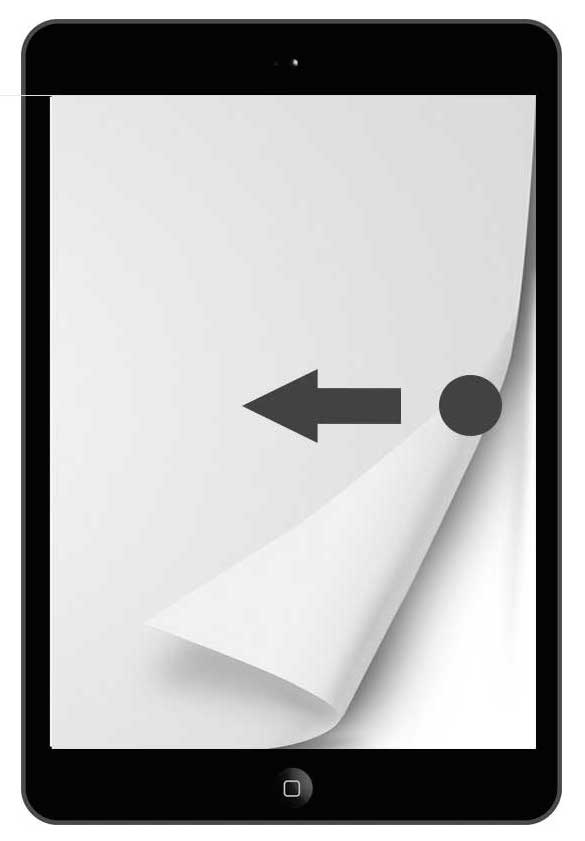
\includegraphics[scale=0.3]{Flip-1.jpg}
    \caption{Single Finger Flip}
    \label{fig:Flip-1}
\end{figure}

\begin{figure}[!hb]
    \centering
    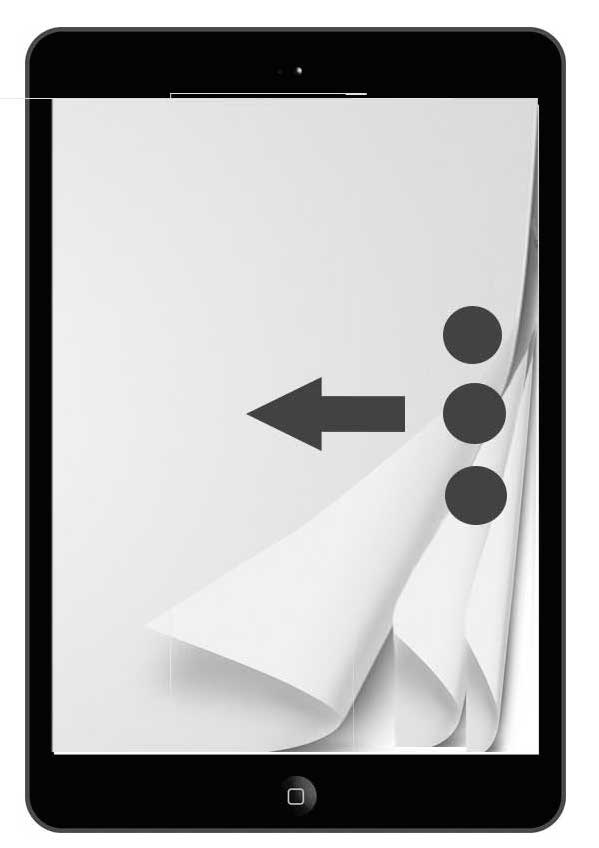
\includegraphics[scale=0.3]{Flip-2.jpg}
    \caption{Three Finger Rifling}
    \label{fig:Flip-2}
\end{figure}

\begin{figure}[!hb]
    \centering
    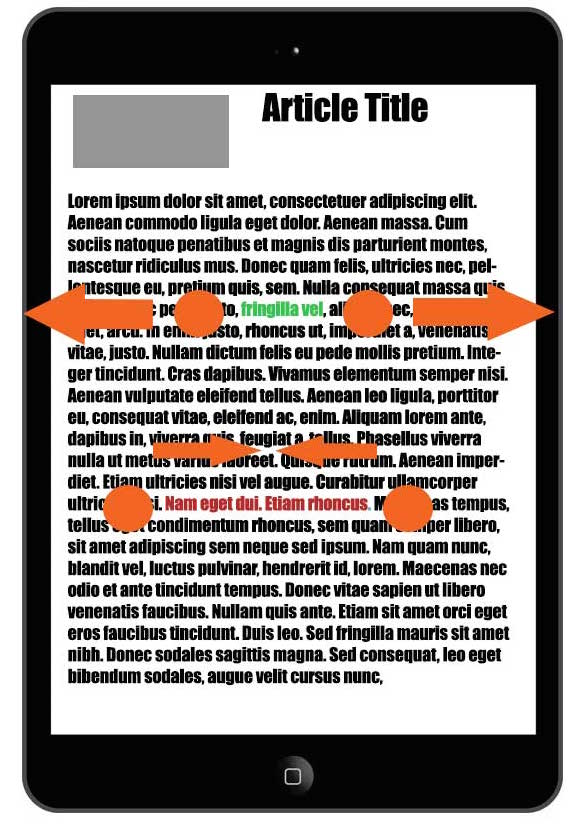
\includegraphics[scale=0.3]{Saving-Pinches.jpg}
    \caption{Pinch To Save}
    \label{fig:Saving-Pinches}
\end{figure}

\begin{figure}[!hb]
    \centering
    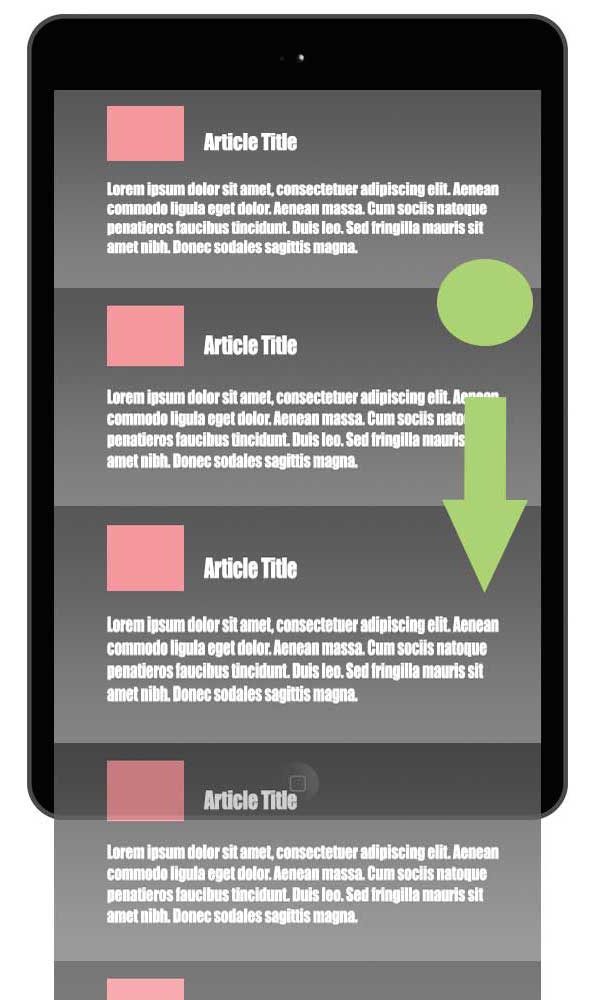
\includegraphics[scale=0.3]{Endless-List.jpg}
    \caption{Endless Vertical Scrolling}
    \label{fig:endless-scroll}
\end{figure}

\begin{figure}[!hb]
    \centering
    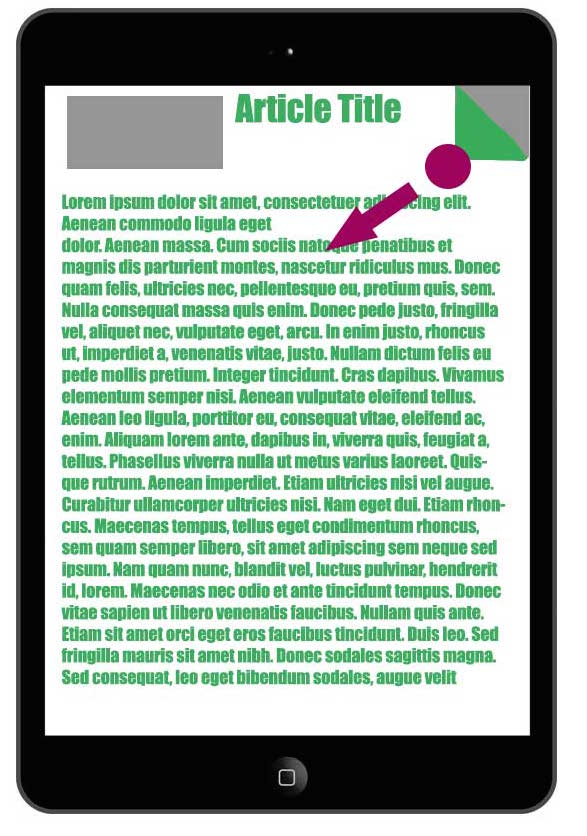
\includegraphics[scale=0.3]{dog-ear.jpg}
    \caption{Dog-Earring}
    \label{fig:dog-earring}
\end{figure}

\begin{figure}[!hb]
    \centering
    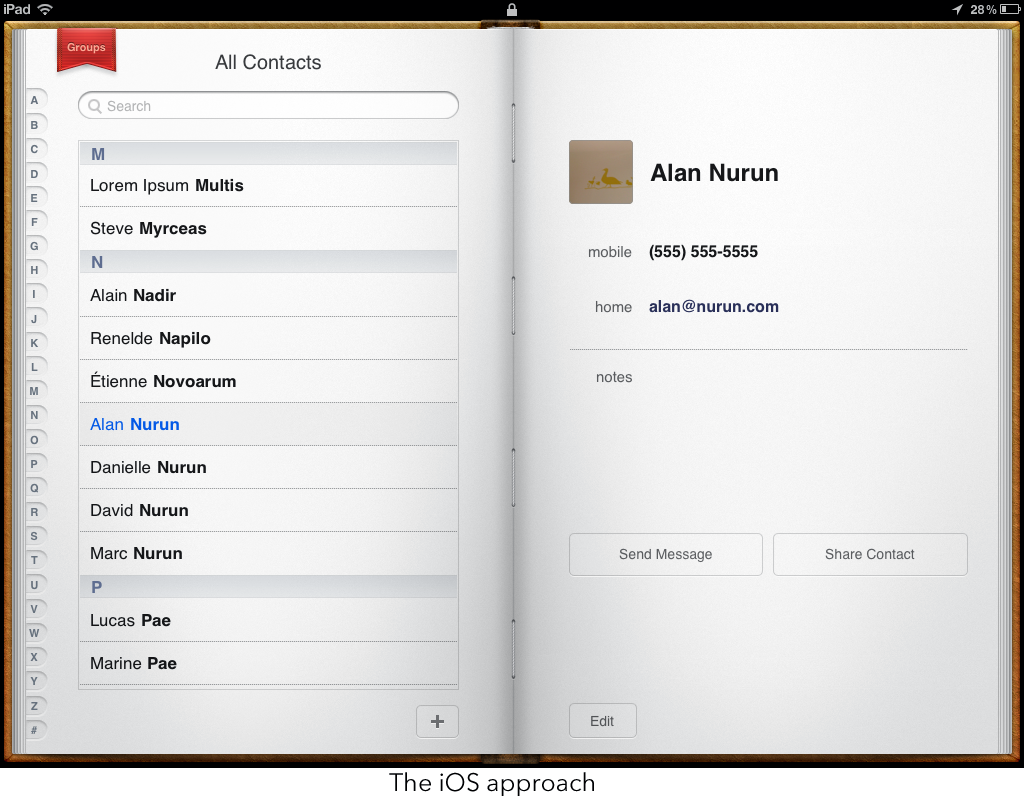
\includegraphics[scale=0.3]{apple-skeu.png}
    \caption{Skeumorphism}
    \label{fig:apple-skeu}
\end{figure}



\end{document}  